%!TEX root = ../march2025poster.tex

\begin{block}{Methods (cont.)}
\textbf{Step 3: Predict parameters using climate and population data}
\begin{itemize}
	\item Calculate the population density ($x_1$), percent of people under 18 ($x_2$), latitude ($x_3$), mean maximum temperature ($x_4$), mean maximum relative humidity ($x_5$), mean minimum relative humidity ($x_6$), and mean average absolute humidity ($x_7$) for each state and flu season, using census population data and gridMET climate data 
	\item Use Monte Carlo Markov Chain methods in Stan to fit the following statistical model $$y_k \sim \alpha_k + \sum_{i=1}^7 \beta_{ik}x_i + \text{Normal}(0, \sigma_k)$$ for $k = 1,2,3,4$, where $y_1=$ up slope, $y_2=$ down slope, $y_3=$ peak week, and $y_4=$ peak value
	\item Use $\alpha_k$ and $\beta_{ik}$ to predict the piecewise linear fit for each flu season and state based on the climate and population variables for that season/state and compare to the actual fit
\end{itemize}	

\end{block}

\vspace{\coltwosep}

\begin{block}{Results (so far)}
	\begin{center}
		\begin{figure}
			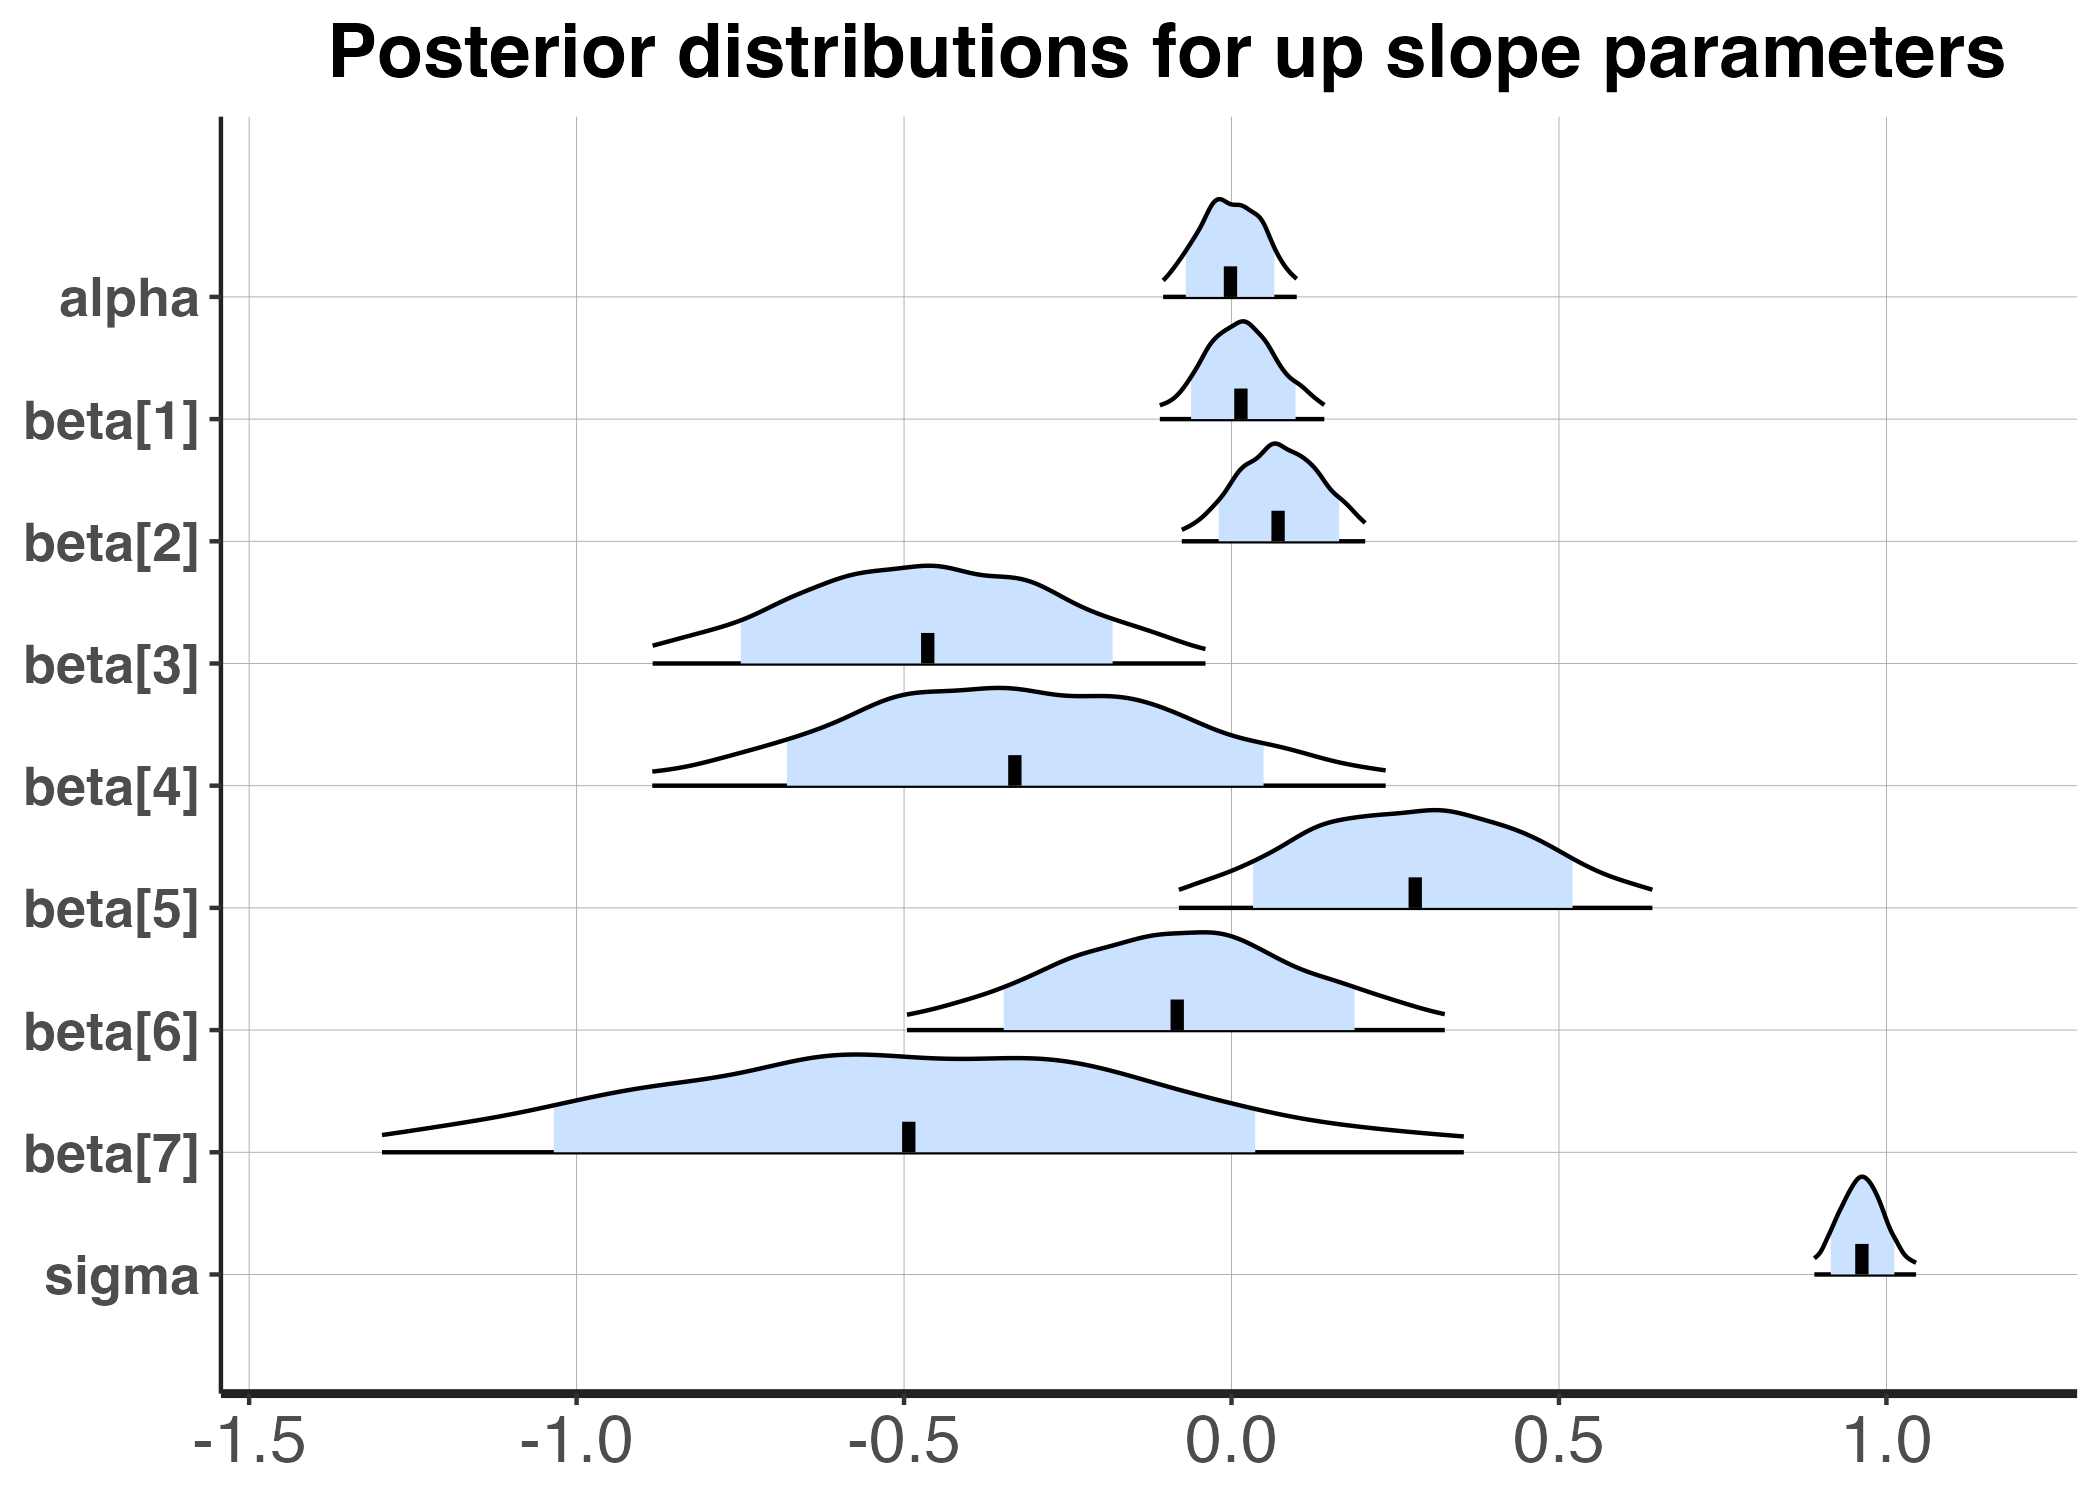
\includegraphics[width = 0.48\columnwidth]{sections/images/upslope_plot.png}
			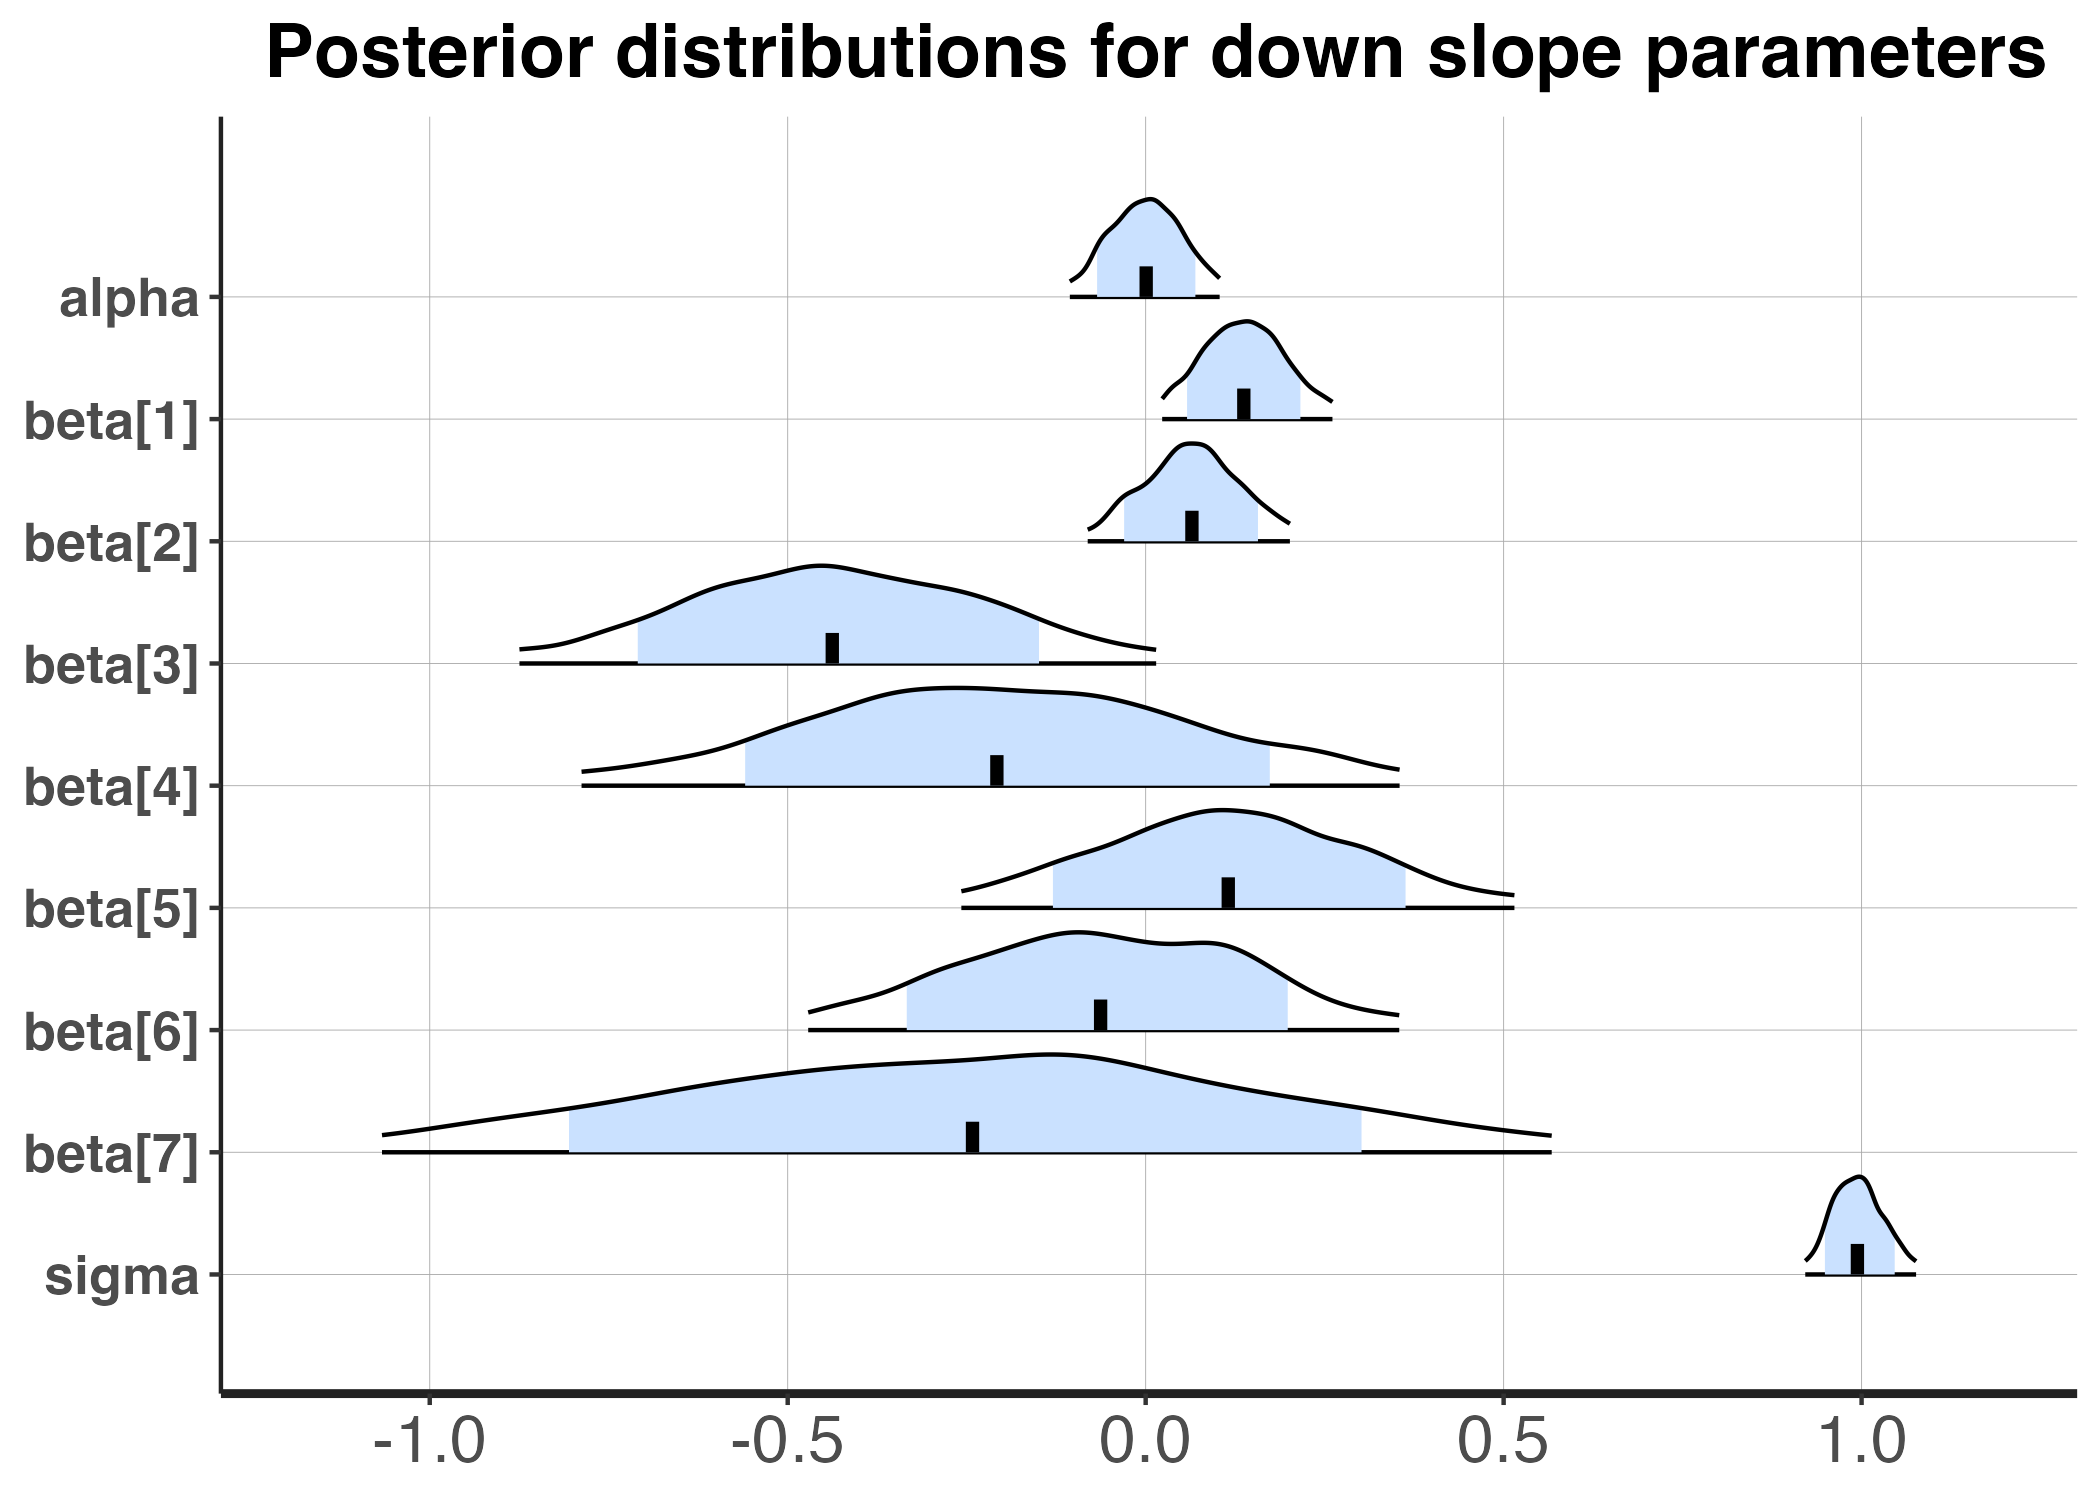
\includegraphics[width = 0.48\columnwidth]{sections/images/downslope_plot.png}
			\\
			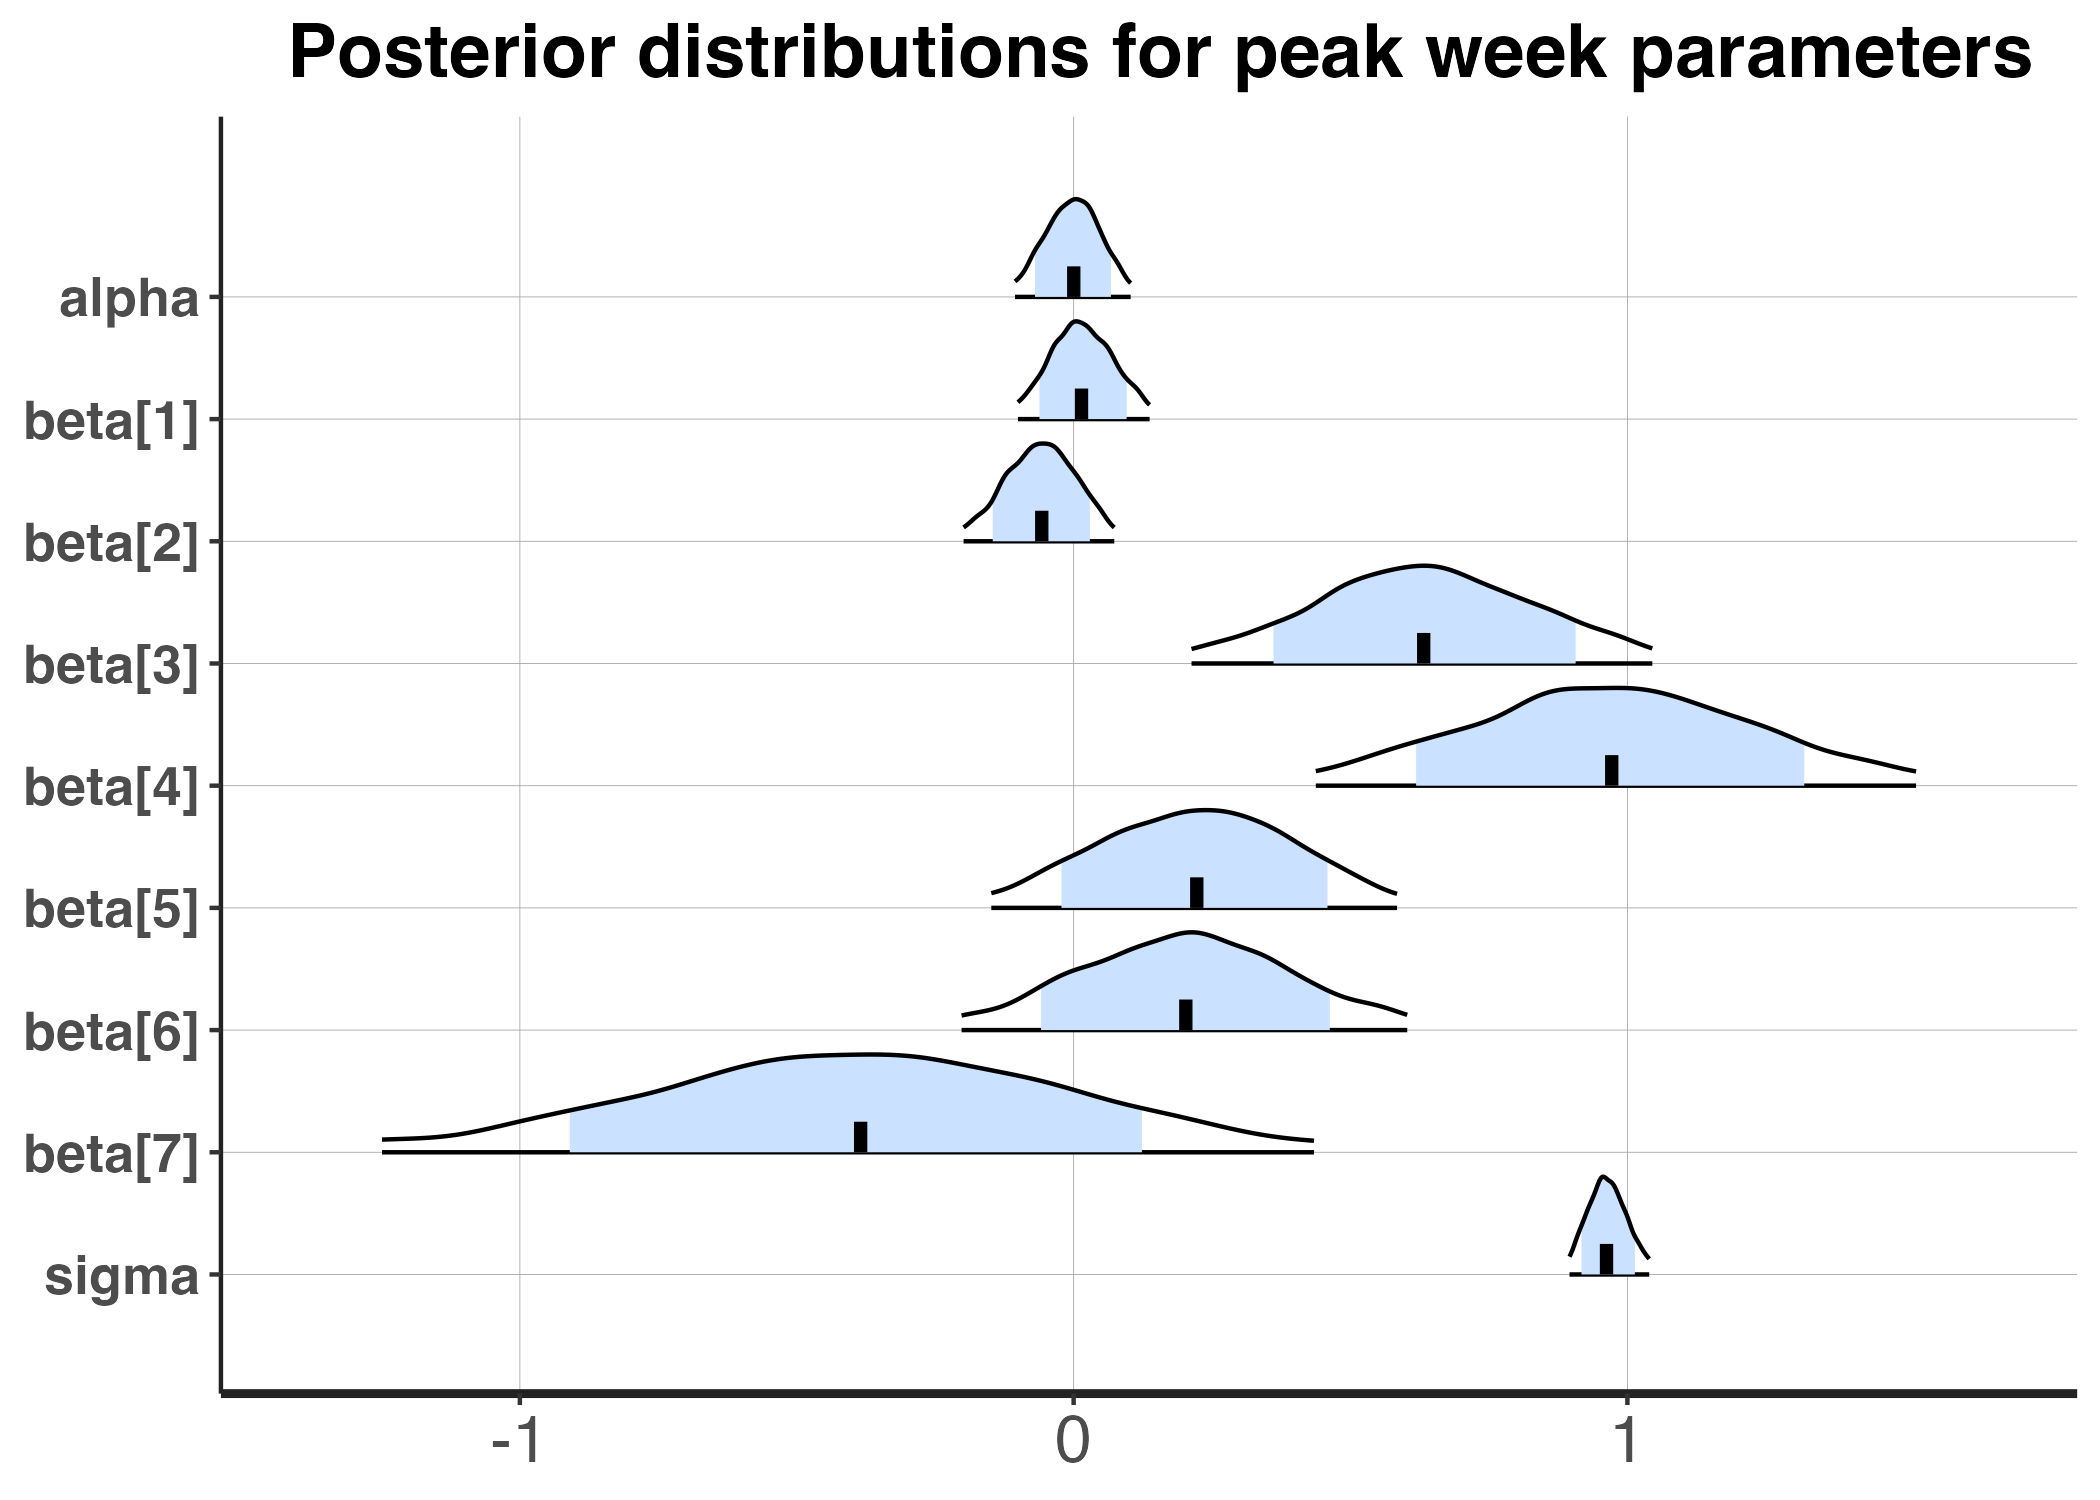
\includegraphics[width = 0.48\columnwidth]{sections/images/peakwk_plot.png}
			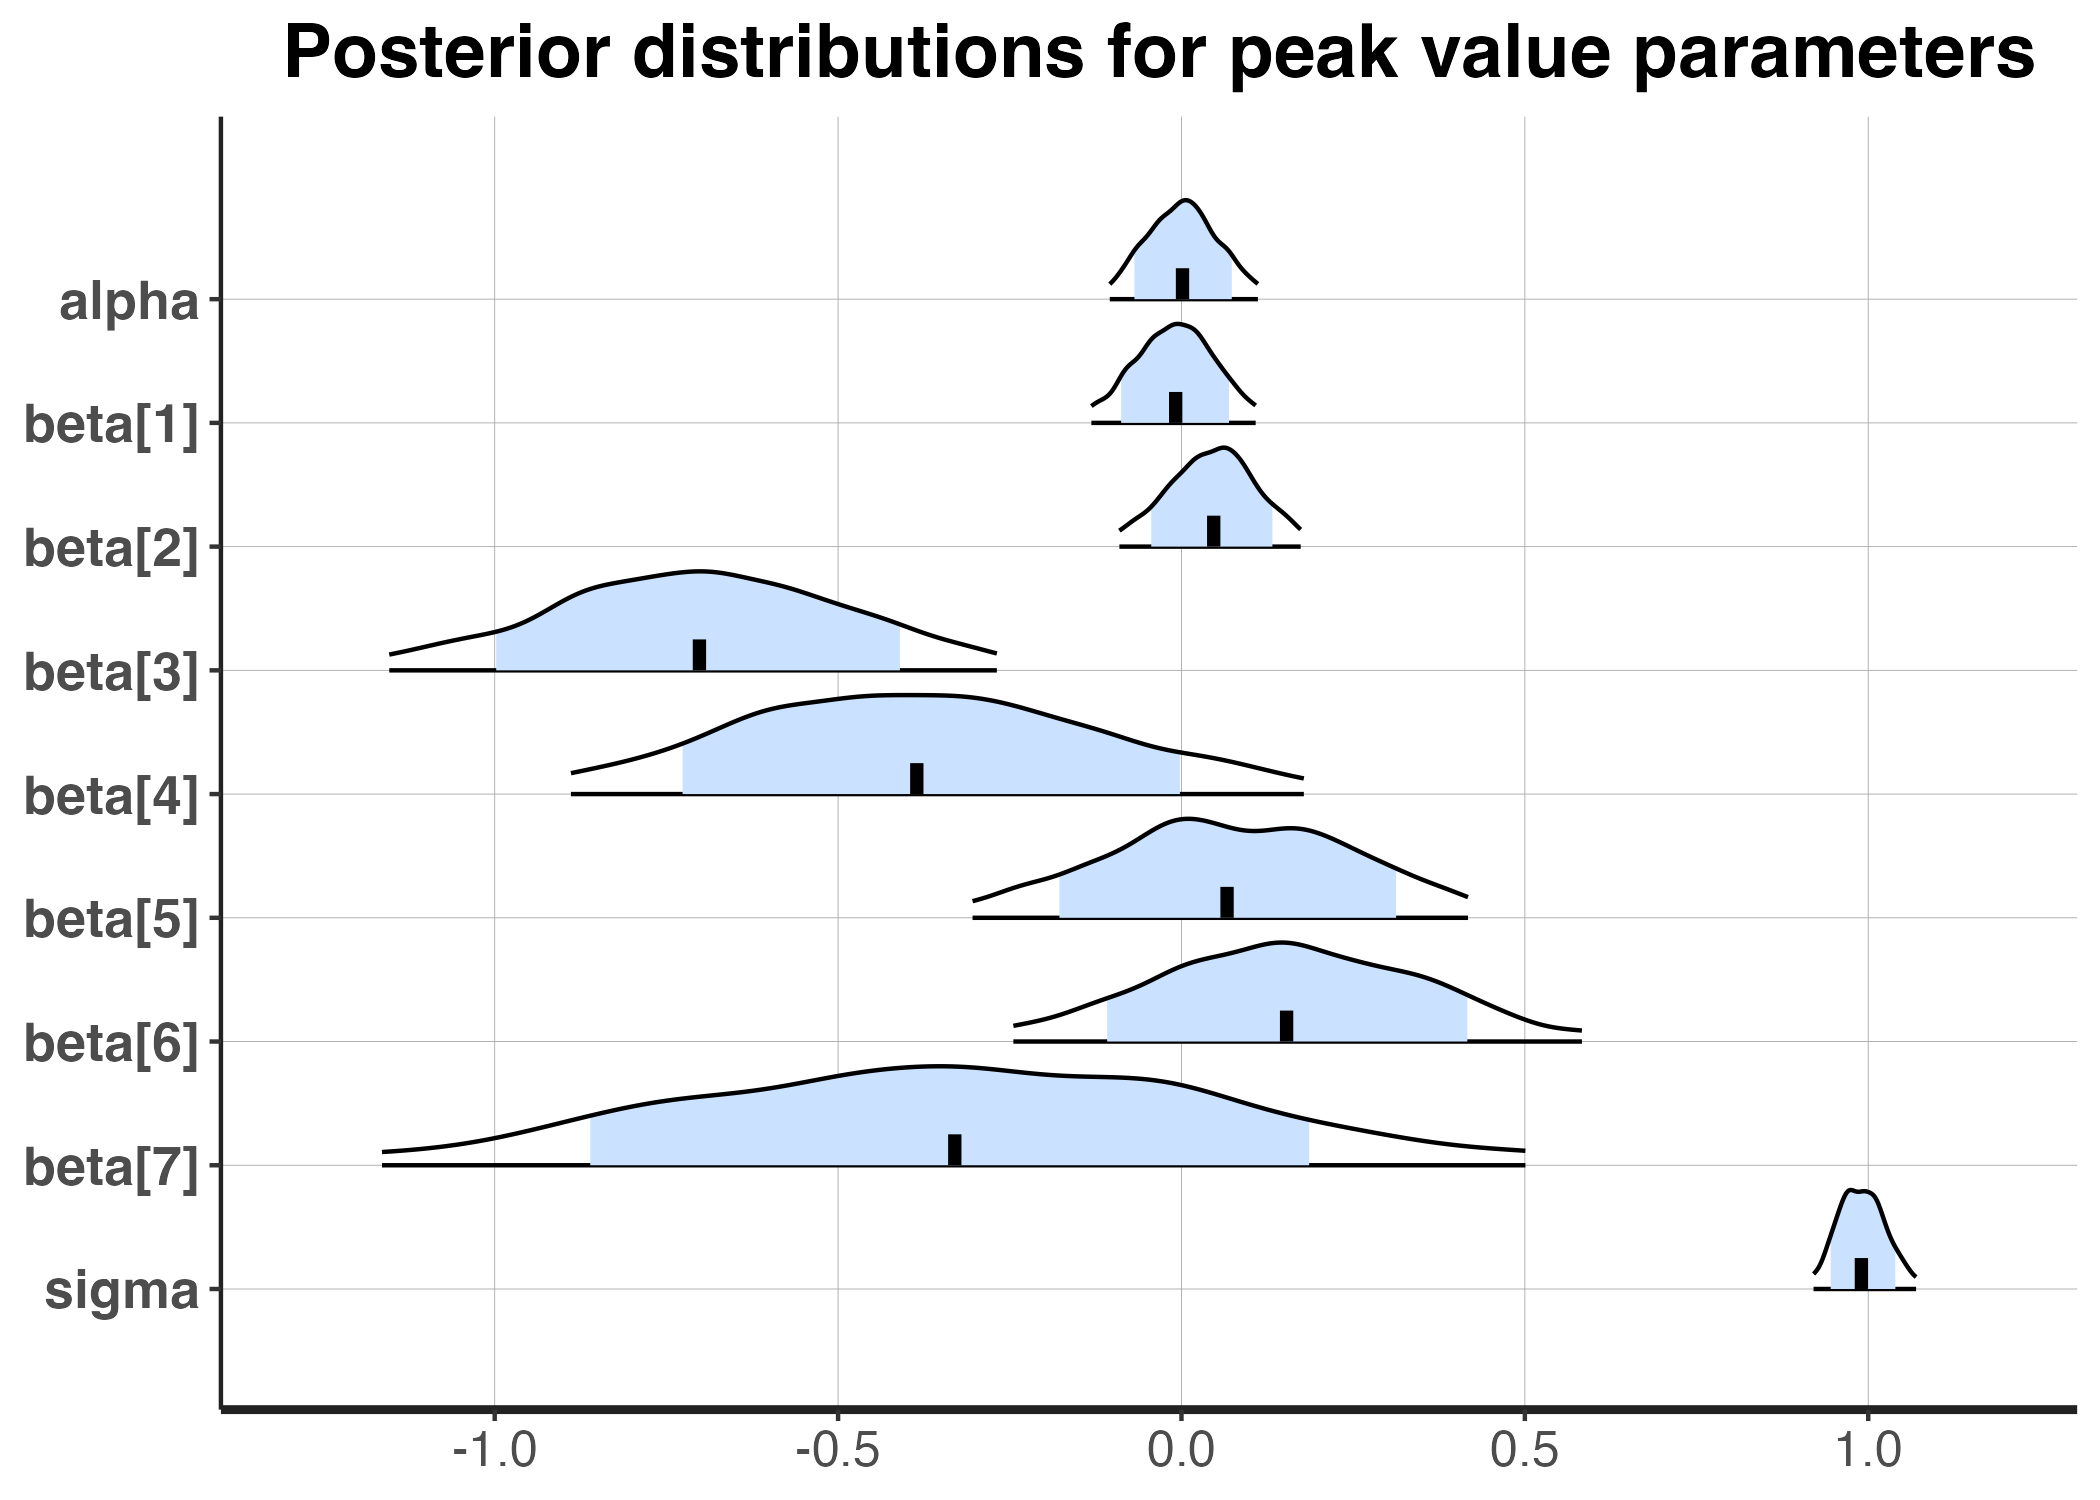
\includegraphics[width = 0.48\columnwidth]{sections/images/peakval_plot.png}\\
			\caption{Posterior distributions for $\alpha_k, \beta_{ik}, \sigma_k$ parameters for up slope, down slope, peak week, and peak value. The blue shaded regions are $80\%$ credible intervals and the total lines plotted are $95 \%$ credible intervals.}
		\end{figure}
	\begin{itemize}
		\item Overall $\beta_3$, which corresponds to latitude, is the most significant
		\item The further north a state is, the less steep their up slope tends to be, the steeper their down slope tends to be, the later their peak week tends to be, and the smaller their peak value tends to be
		\item The more dense a state is, the less steep their down slope tends to be
		\item The hotter a state is in a given year, the later their peak week tends to be
	\end{itemize}
	\end{center}

\end{block}

